This example demonstrates 

Consider a Timoshenko cantilever beam fixed at $x=0$ and loaded with a transverse force $\bar{F} \FrameBasis_z$ at the free end $x=L$.

\subsubsection{Rectangle}

\paragraph{Shear correction}

Consider the following cases:
\begin{description}
    \item[Case II: Plane Stress]
    \item[Case II: ]
\end{description}



\paragraph{Discussion}
\cite{puchegger2003experimental} found that the $\kappa$-factor decreases with increasing depth-to-width ratio, and that dependence on the aspect ratio increases with increasing Poisson’s ratio.

This example was considered by \cite[5.2.1]{saritas2006mixed}.



\subsubsection{Hollow Rectangle}\label{sec:frame-0012/H}
\begin{figure}[H]
    \centering
    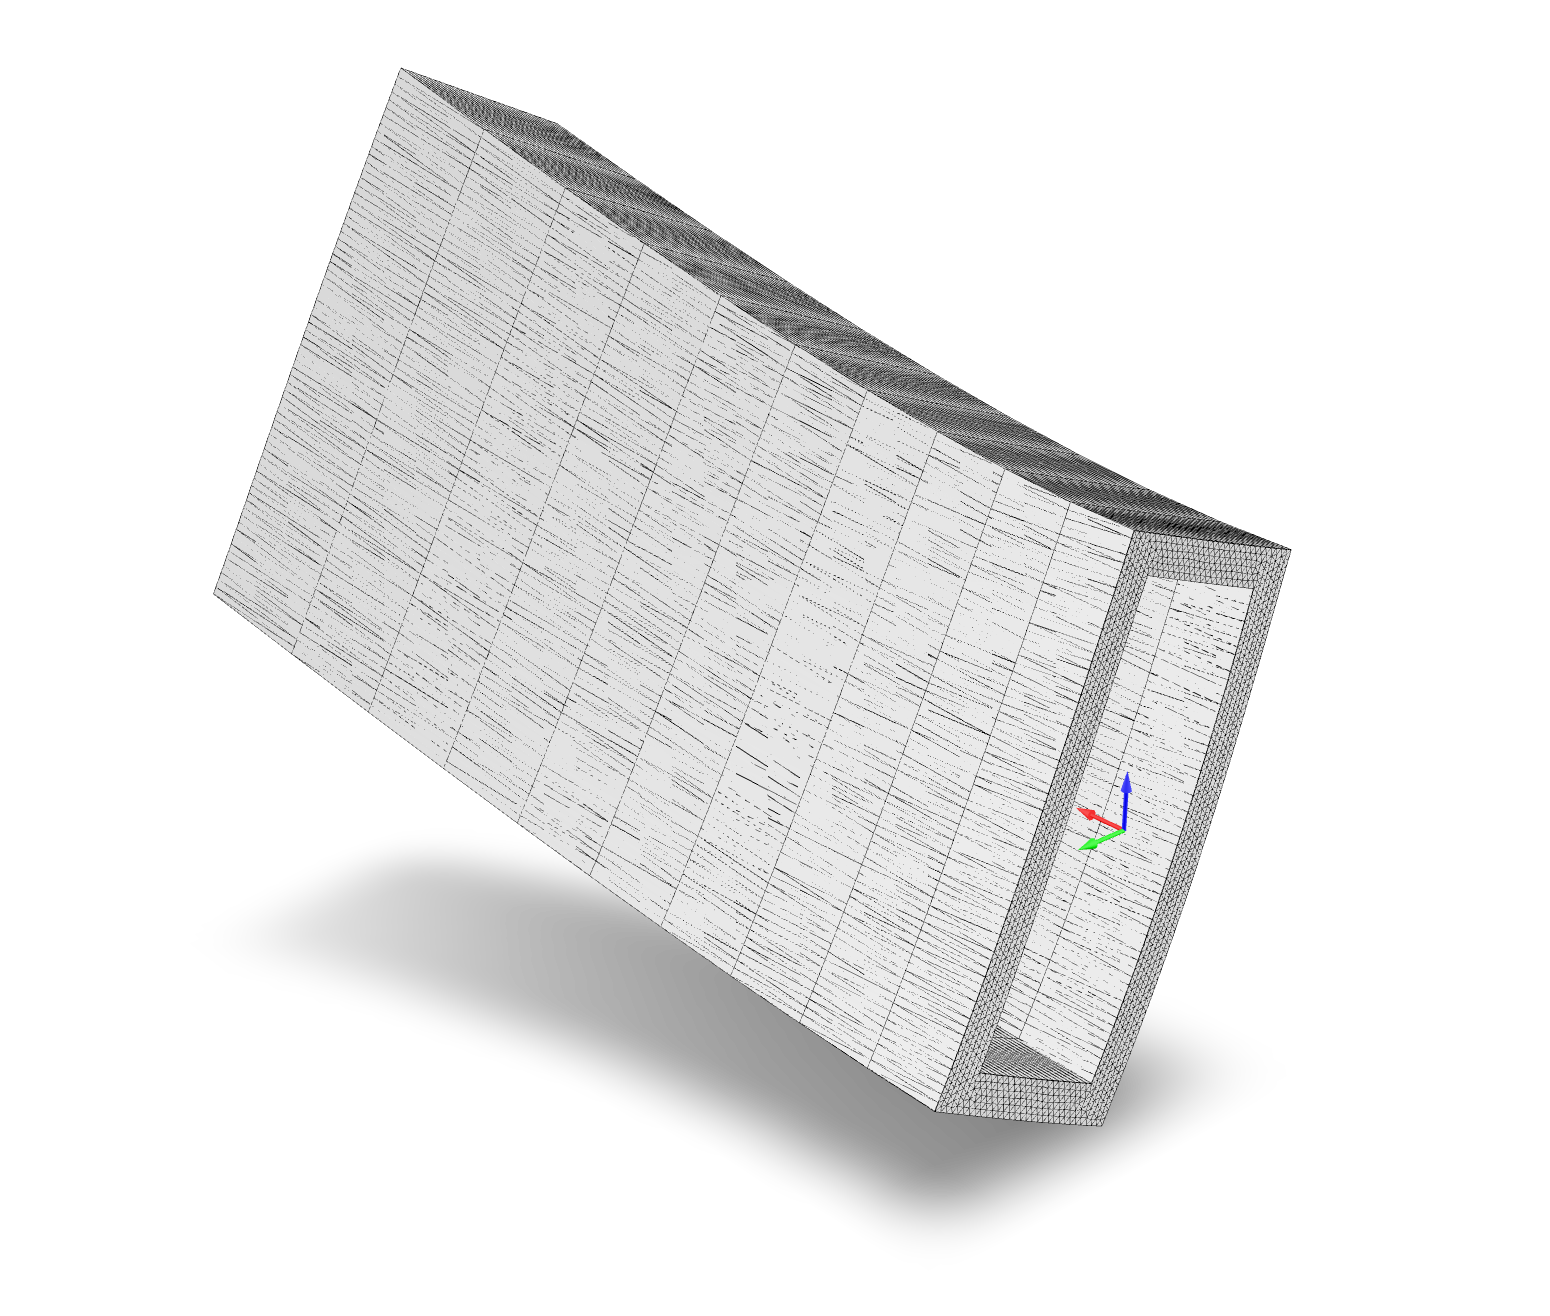
\includegraphics[width=0.5\linewidth]{Examples/frame-0012/img/0012-tube-soln.png}
    \caption{Continuum solution from Example~\ref{sec:frame-0012/H}}
    \label{fig:0012-tube}
\end{figure}

\cite{cowper1966shear}:
\begin{equation*}
\frac{10(1+\nu)(1+3 m)^2}{\left(12+72 m+150 m^2+90 m^3\right)+\nu\left(11+66 m+135 m^2+90 m^3\right)+10 n^2\left((3+\nu) m+3 m^2\right)},
\end{equation*}
where
\[
m=\frac{b t_1}{h t_2} \text { and }
n=\frac{b}{h}
\]


\subsubsection{Wide Flange}\label{sec:frame-0012/w}

\FrameSection{
  label/problem={frame-0012/w},
  kinematics/section={\eqref{eq:linear-gl-strain-pi}},
  A=11.78,
  Iy=613.8,
  label/shape=W18x40,
  unit/length=\inch,
  %
  E=29e3,
  material=Steel,
  unit/stress=\si{\psi}
}
\begin{table}[H]
    \centering
    \caption{Computed properties for a \emph{W18x40} wide flange section}
    \label{tab:w18x40-properties}
\end{table}


\subsubsection{Channel}
\cite{paradiso2021shear}

\subsubsection{Angle}\label{sec:frame-0012/A04}
\begin{figure}[H]
    \centering
    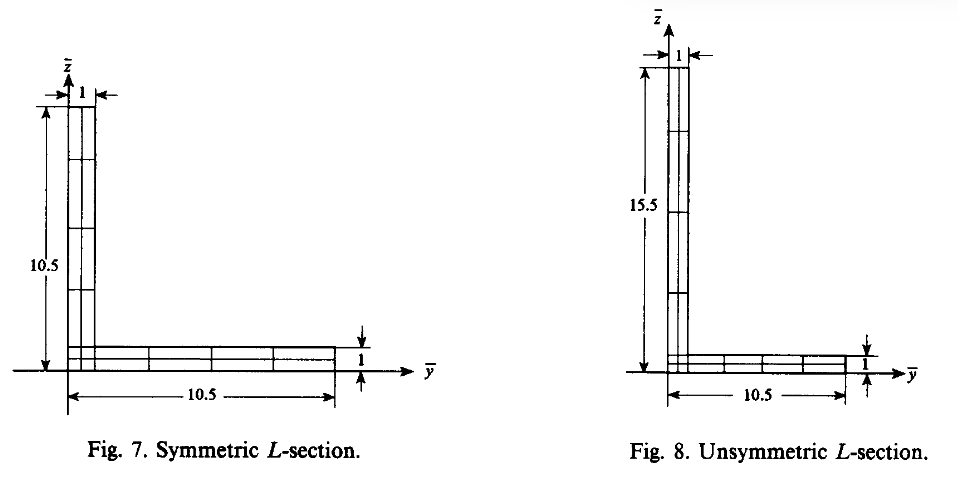
\includegraphics[width=0.75\linewidth]{Examples/frame-0012/schramm-angles.png}
    
\end{figure}
\cite{schramm1994shear} and \cite{dong2010much}

\subsubsection{Bridge Girder}\label{sec:frame-0012/G02}
This example is considered by \cite{gruttmann2001shear,tran2021efficiency}.
\begin{figure}[H]
    \centering
    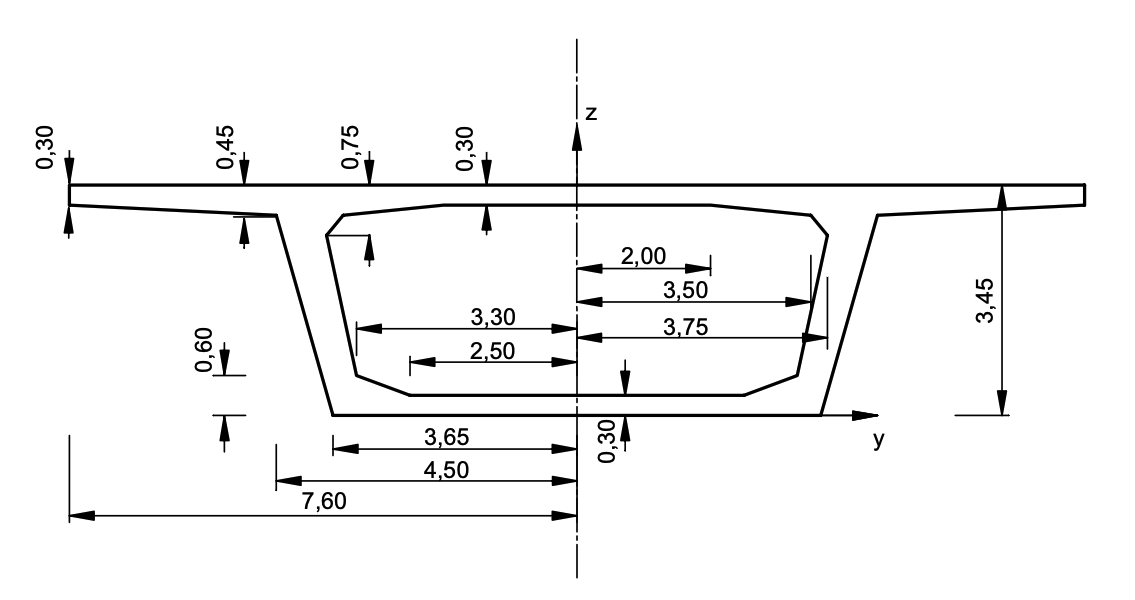
\includegraphics[width=0.75\linewidth]{Figures/SimpleGirder.png}
    \caption{Girder section from Example~\ref{sec:frame-0012/G02}.}
    \label{fig:single-girder}
\end{figure}
